\documentclass[10pt]{article}
\usepackage[a4paper,margin=2.1cm,top=2.2cm,bottom=2.4cm]{geometry}
\usepackage[T1]{fontenc}
\usepackage{lmodern}
\usepackage{microtype}
\usepackage{amsmath,amssymb}
\usepackage{graphicx}
\usepackage{booktabs,tabularx,array}
\usepackage{xcolor}
\usepackage{enumitem}
\usepackage{float}
\usepackage[font=small,labelfont=bf]{caption}
\usepackage{tikz}
\usetikzlibrary{arrows.meta,positioning,shapes.geometric,fit,calc}
\usepackage[colorlinks=true,linkcolor=fdgreen,citecolor=fdgreen,urlcolor=fdgreen]{hyperref}

\definecolor{fdgreen}{HTML}{1F9D55}
\definecolor{fdink}{HTML}{1D2B24}
\definecolor{fdmute}{HTML}{8A958F}
\definecolor{fdred}{HTML}{C8473B}
\definecolor{fdpale}{HTML}{E8F5EE}
\setlist{nosep,leftmargin=1.4em}
\setlength{\parskip}{3pt}
\newcommand{\code}[1]{\texttt{\small #1}}
\newcommand{\mon}{\textsc{mon}}
\newcommand{\tx}[2]{\href{https://testnet.monadvision.com/tx/#1}{\code{#2}}}
\graphicspath{{fig/}}

\title{\vspace{-1em}\textbf{PRESENCE: Server-Timed, Motion-Witnessed Proof of Human Process on Monad}\\[4pt]
\large with FACEDOWN, a phone-free commitment app, and Knock to Approve for AI agents}
\author{Team WARRIO: Aaditya (lead, \href{https://github.com/Aaditya1273}{github.com/Aaditya1273})\\ and
arpit\_1 (co-founder, \href{https://github.com/lsuDOKO}{github.com/lsuDOKO})\\[2pt]
\small Technical whitepaper \;$\cdot$\; 15 October 2026\\
\small Monad testnet (chain 10143) \;$\cdot$\; \code{PresenceRegistry} \code{0x5519dacf\ldots E52B}\\
\small Source: \url{https://github.com/notwen123/PRESENCE} \;$\cdot$\; Film: \url{https://youtu.be/XANOR8fdU4E}}
\date{}

\begin{document}
\maketitle
\vspace{-1.6em}

\begin{abstract}
\noindent Commitment devices for phone use rely on things that cannot be checked: a local timer, a screenshot, or a human
reviewer. Software can fake all three, and AI agents can now operate a phone. PRESENCE is a verification engine that
turns ``this person left their phone alone for $D$ minutes'' into a record that is checked by a server and anchored on
Monad. A session is a server-timed sequence of $N$ windows. Each window carries one presence check at a moment the user
cannot predict. The user answers it by knocking on the back of the face-down phone. Each window seals a checkpoint into a
SHA-256 hash chain signed by an ephemeral Android Keystore key bound into a Sign-In-With-Ethereum (EIP-4361) message,
which the user's wallet signs: a Privy embedded wallet created when the user signs in with Google. The checkpoint
contains two accelerometer summaries: the share of the window the phone lay still and face-down ($\pi$), and the largest
physical jolt felt within 300\,ms of the answer ($\mu$). The ATTEST server re-derives the chain and evaluates a
nine-clause predicate on its own clock. It then writes a create-once record to the \code{PresenceRegistry} contract,
where any contract can ask \code{isPresent()} or \code{presentDays()}, and only after that record confirms pays out from
\code{PresenceVault}. FACEDOWN, the first app, offers three modes: \emph{Free} (sponsor-paid), \emph{No-Loss} (the stake
always comes back) and \emph{Stake} (a quitter's stake is locked for 7/14/30 days, never taken). Nobody's money is ever
paid to another user. The same physical check gates AI agents: in \emph{Knock to Approve}, an agent (a Privy server
wallet that a Privy policy confines to the \code{AgentGuard} contract) spends up to 0.01\,\mon{} alone, and any larger
transfer waits for a P-256 signature from its human's phone, given by a knock and verified on-chain through Monad's
RIP-7212 precompile.

\emph{Results.} Measurements from the earlier devnet prototype (9--12 October 2026, a real Android phone and the
emulator): 56 sessions from 20 wallets, 19 settled and 9 rejected. The timing heuristic scored all 22 sessions that had
enough answers at risk $0$, including every session driven by \code{adb input tap}. Timing alone does not detect a
script. The motion floor $\tau=150$\,mm/s$^2$ did: \textbf{29 of 30} injected taps on the real phone read
20--115\,mm/s$^2$ (median 35.5). One read 734\,mm/s$^2$. Every one of the eight injected-tap sessions contains at least one
reading below the floor and would be rejected in production. The emulator's synthetic knocks (2,189--2,190\,mm/s$^2$)
\emph{pass}. This shows that a client able to inject sensor values defeats the motion check, and hardware attestation is
required to close it. On Monad testnet, recording one verified session cost 161,016 gas ($\approx$0.0164\,\mon{} at
102\,gwei; 13 Oct) and, in a later measurement, 128,512 gas (0.0131\,\mon{}, $\approx$\$0.0003 at \$0.0244/\mon{};
14 Oct); blocks averaged 0.304\,s. Real-phone sessions with Google sign-in through Privy, a No-Loss stake, and Knock to
Approve with a physical knock are on-chain. Re-deriving the chain and evaluating the policy takes 16\,\textmu s (median)
for a 4-checkpoint session on a laptop CPU. The system comprises about 2,600 lines of Python, 355 lines of Solidity and
about 5,400 lines of Kotlin, with 59 backend tests, 10 Foundry contract tests (including real P-256 signatures) and 10
Android unit tests passing. Nothing here is on mainnet; all value is testnet \mon{}.
\end{abstract}

\noindent\textbf{Keywords:} proof of human process, commitment devices, Monad, EVM, Privy, P-256 / RIP-7212,
human-in-the-loop AI agents, accelerometer liveness, hash-chained evidence, loss aversion without forfeiture

\section{Introduction}

Phones are built to be picked up. Blocking apps help, but they can be undone at the exact moment of the urge.
\emph{Commitment devices}, where you put something at stake on your own future behaviour, are among the best-studied
tools in behavioural economics. They have a structural weakness on phones, though: someone must decide whether the
commitment was kept. Today that someone is a local timer the user controls, a photo a human or model reviews, or the
user's own word. None of these can back money. A timer can be fast-forwarded. A photo can be staged. A model reviewer
costs money on every claim. There is also a newer problem. Agents that operate phone interfaces can now complete login
and approval flows on their own~\cite{liu2026}. Any reward that only checks for taps on a screen can be farmed by one,
and any wallet an agent controls can be drained by one.

We ask a narrow question: \emph{can a phone produce evidence, strong enough to settle a financial commitment, that a
person left it alone for a stated time and was physically there to answer when asked?} PRESENCE answers it with three
design choices:
\begin{enumerate}
\item \textbf{The server keeps time.} Every duration and gap is measured on the ATTEST server's clock. Client timestamps
are informational.
\item \textbf{The check-in is physical.} A presence check appears at a random moment in each window. The user answers it
by knocking on the back of the face-down phone, and the accelerometer must feel the knock. An injected tap moves nothing.
\item \textbf{The verdict is recorded once.} A \code{PresenceRegistry} entry keyed by (identity, mission, day, sequence)
can be written exactly once. A payout is sent only after that write confirms.
\end{enumerate}

\subsection{Contributions}
\begin{itemize}
\item A \textbf{commitment calculus} (\S\ref{sec:calculus}): a validated mission policy, a nine-clause server predicate
evaluated on the server clock, a closed-form automation risk score, and two accelerometer statistics with exact
definitions.
\item A \textbf{hash-chained, key-bound evidence format} (\S\ref{sec:evidence}). It is byte-identical in Kotlin and
Python, shares golden vectors between them, and puts only 32 bytes on-chain.
\item \textbf{Loss aversion without forfeiture} (\S\ref{sec:econ}). A cool-down lock replaces stake confiscation, so
nobody ever wins anyone else's money. We give its expected cost next to forfeiture-based devices, plus pool accounting
that cannot pay out more than sponsors deposited.
\item \textbf{Monad contracts} (\S\ref{sec:chain}): a create-once registry that any contract can query for recent and
sustained presence, a vault for stakes and sponsor rewards, and an airdrop that pays only identities present on enough
distinct days.
\item \textbf{Knock to Approve} (\S\ref{sec:agentguard}): a human-in-the-loop limit for AI agents, where a transfer above
the limit needs a P-256 signature from a bound phone, verified by the contract itself.
\item \textbf{Measurements} from the earlier devnet prototype and from live Monad testnet transactions with a real phone
(\S\ref{sec:eval}). They include a negative result: our timing heuristic alone does not detect a scripted client.
\item A \textbf{limitations list ranked by severity} (\S\ref{sec:limits}), including the attacks that defeat the
current build.
\end{itemize}

\section{Evidence Behind the Design}\label{sec:evidence-base}

FACEDOWN's product decisions follow from published randomised and measurement studies. Table~\ref{tab:evidence} maps
each one to the mechanism it motivated. Every number is quoted from the paper's abstract.

\begin{table}[h]\small
\caption{Published findings and the design decision each produced.}\label{tab:evidence}
\begin{tabularx}{\linewidth}{@{}X X@{}}\toprule
\textbf{Finding} & \textbf{Decision in FACEDOWN} \\\midrule
Deposit contracts were accepted by 13.7\% of smokers versus 90.0\% for reward programs ($n=2{,}538$). Among those who
would accept either, deposits raised abstinence by 13.2 points~\cite{halpern2015}. &
Free (sponsor-paid) first. No-Loss as the default way to put money in. Stake is opt-in for the committed. \\
Appointments more than doubled HIV-testing rates compared with financial commitment devices, and most takers of the
latter lost their money~\cite{derksen2021}. &
A daily \emph{facedown appointment} with a reminder. Failure never costs principal. \\
Self-selected phone-reduction goals cut use by 26\,min/day more (a 73\% larger reduction) than assigned goals (RCT,
$N=149$, 12 weeks)~\cite{sachdeva2026}. &
The user chooses the length (2, 10, 25, 60\,min) and what is at stake. \\
A month-long RCT blocking mobile internet for two weeks improved sustained attention, mental health and well-being; 91\%
improved on at least one outcome~\cite{castelo2025}. &
A \emph{Facedown Hour}, not only short timers. A passive all-day ring (Presence Minutes). \\
A pause before opening a target app (the \emph{one sec} self-nudge) reduced actual openings by 57\%~\cite{gruning2023}. &
\emph{Urge Catcher}: the pause, plus an offer of a 10-minute verified session in place of the app. \\
Group-pooled incentives produced 3.2\,kg more weight loss than individual incentives (95\% CI 0.9--5.5)~\cite{kullgren2013}. &
\emph{Squads} of 3--8 share one streak. \\
A motion-based signal distinguished human from agent-driven logins with 98.4\% (table-top) and 92.6\% (hand-held)
accuracy over 116 pilot sessions~\cite{liu2026}. zkSENSE reached 92\% humanness accuracy from motion sensors~\cite{zksense}. &
Knock check-ins and face-down stillness in every checkpoint. \\
In 9 of 12 NFT play-to-earn games, players who traded had a negative profit on average~\cite{gao2026}. &
No new token and no emissions. Rewards come only from sponsor deposits. \\
Sustaining $s$ identities over $T$ windows requires at least $sT/\tau_h$ participation channel-windows when
participation must be re-earned per identity per window~\cite{bpc2026}. &
\code{presentDays()} and \code{SustainedHumanAirdrop}: eligibility needs presence on many distinct days, not once. \\\bottomrule
\end{tabularx}
\end{table}

\section{Threat Model and Design Goals}\label{sec:threat}

\paragraph{Principals.} The \emph{user} runs the FACEDOWN Android app and signs in with Google through Privy, which
creates a self-custodial embedded EVM wallet on Monad testnet; that wallet signs the session's SIWE message and the stake
transaction inside the app (builds without Privy credentials fall back to MetaMask). The \emph{ATTEST} server issues
nonces, keeps time, verifies evidence, decides, and sends settlements with the attestor key. The \emph{contracts} on
Monad record attestations and pay out, and accept those writes only from the configured attestor. \emph{Sponsors} fund
rewards in \mon{} through \code{PresenceVault.fund()}. For Knock to Approve, an \emph{AI agent} acts through a Privy
server wallet, and the user's phone holds a P-256 key bound to an \code{AgentGuard} account.

\paragraph{Adversary.} The adversary is the user, or anyone acting for them, who wants a VERIFIED verdict (and its
reward or returned stake) without leaving the phone alone. They control the phone's software. They can modify or
re-sign the APK, replay traffic, run many wallets, drive the UI from \code{adb}, an accessibility service or an AI phone
agent, and alter the stake transaction inside a wallet. They do not control the ATTEST server, its clock or the attestor
key. They cannot forge ECDSA signatures (secp256k1 or P-256) or find SHA-256 collisions. In the version described here
they \emph{can} inject accelerometer values if they run a modified OS or an emulator (\S\ref{sec:limits}). For Knock to
Approve, the adversary is a compromised or misbehaving agent, or a relay that wants to approve a transfer the human did
not.

\paragraph{Goals.}
\begin{enumerate}[label=\textbf{G\arabic*}]
\item \textbf{Duration integrity.} A session cannot verify in less than its stated wall-clock time as measured by the
server.
\item \textbf{Continuity.} The app must stay in the foreground in every window. A missed window is visible.
\item \textbf{Physical presence.} Each answer is accompanied by a physical jolt of the device, and the device lay
face-down and still for most of each window.
\item \textbf{Evidence integrity.} Checkpoints cannot be reordered, dropped, replayed into another session or edited
after sealing.
\item \textbf{Single claim.} A device's identity can claim a mission at most $c_{\max}$ times per UTC day. A claim's
payout cannot be repeated.
\item \textbf{Principal safety.} No verdict transfers one user's stake to another user.
\item \textbf{Human-gated agents.} An agent cannot move more than its per-transfer limit without a fresh signature from
its human's bound phone, and cannot sign transactions to any contract other than \code{AgentGuard}.
\end{enumerate}

\paragraph{Non-goals.} We do not prove that the person is the wallet owner or one unique human (proof of personhood).
We do not prove what the person was doing while away from the phone. We cannot stop the use of a second phone.

\section{System Architecture}\label{sec:arch}

\begin{figure}[t]\centering
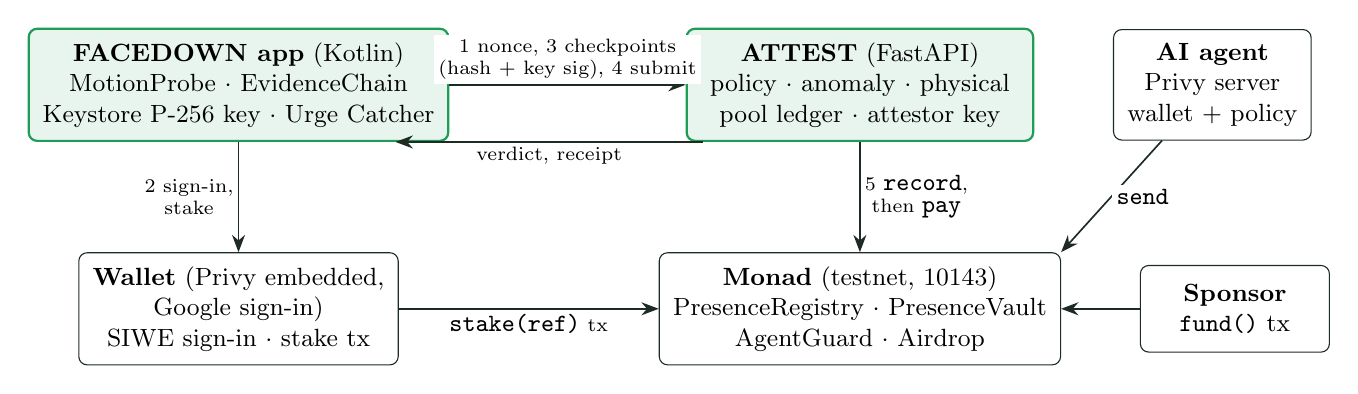
\begin{tikzpicture}[font=\small, node distance=6mm and 10mm,
  box/.style={draw=fdink, rounded corners=3pt, fill=white, align=center, inner sep=5pt, minimum height=11mm},
  gbox/.style={box, fill=fdpale, draw=fdgreen, line width=.8pt},
  lab/.style={font=\scriptsize, align=center, fill=white, inner sep=1.5pt},
  arr/.style={-{Stealth[length=2.2mm]}, line width=.6pt, draw=fdink}]
\node[gbox, minimum width=40mm] (app) {\textbf{FACEDOWN app} (Kotlin)\\ MotionProbe $\cdot$ EvidenceChain\\ Keystore P-256 key $\cdot$ Urge Catcher};
\node[box, below=14mm of app, minimum width=40mm] (wal) {\textbf{Wallet} (Privy embedded,\\ Google sign-in)\\ SIWE sign-in $\cdot$ stake tx};
\node[gbox, right=30mm of app, minimum width=44mm] (att) {\textbf{ATTEST} (FastAPI)\\ policy $\cdot$ anomaly $\cdot$ physical\\ pool ledger $\cdot$ attestor key};
\node[box, below=14mm of att, minimum width=44mm] (sol) {\textbf{Monad} (testnet, 10143)\\ PresenceRegistry $\cdot$ PresenceVault\\ AgentGuard $\cdot$ Airdrop};
\node[box, right=10mm of att, minimum width=24mm] (agt) {\textbf{AI agent}\\ Privy server\\ wallet + policy};
\node[box, right=10mm of sol, minimum width=24mm] (sp) {\textbf{Sponsor}\\ \code{fund()} tx};
\draw[arr] (app) -- node[lab, above]{1 nonce, 3 checkpoints\\ (hash + key sig), 4 submit} (att);
\draw[arr] (att.200) -- node[lab, below]{verdict, receipt} (app.340);
\draw[arr] (app) -- node[lab, left]{2 sign-in,\\ stake} (wal);
\draw[arr] (wal) -- node[lab, below]{\code{stake(ref)} tx} (sol.west|-wal);
\draw[arr] (att) -- node[lab, right]{5 \code{record},\\ then \code{pay}} (sol);
\draw[arr] (agt) -- node[lab, right]{\code{send}} (sol.north east);
\draw[arr] (sp) -- (sol);
\end{tikzpicture}
\caption{Architecture. The client collects evidence, ATTEST decides, and Monad records the result. The app never
sends \code{verified}, \code{reward} or \code{assurance}. Raw sensor data never leaves the phone.}\label{fig:arch}
\end{figure}

Figure~\ref{fig:arch} shows the components. The rule underneath them is that \emph{authority sits with the party that
cannot be patched by the adversary}. Table~\ref{tab:authority} lists who decides each fact.

\begin{table}[h]\small\centering
\caption{Authority analysis: who decides each fact, and why not the client.}\label{tab:authority}
\begin{tabularx}{\linewidth}{@{}l X X@{}}\toprule
\textbf{Decision} & \textbf{Owner} & \textbf{Reason}\\\midrule
Session nonce & ATTEST & Nonces chosen by the client could be replayed. \\
Wallet identity & ATTEST (EIP-191 signature over the exact SIWE bytes it issued) & The client can be patched. \\
Device identity, claim limit & ATTEST (identity key; on-chain only as its SHA-256 hash) & An address alone proves nothing. \\
Duration and gaps & ATTEST server clock & Client timestamps can be forged. \\
Evidence validity & ATTEST recomputes every hash & --- \\
PASS/FAIL & \code{policy.evaluate} on ATTEST & --- \\
Claim limit, XP, streak, league & ATTEST database (streak mirrored on-chain) & --- \\
Durable record & \code{PresenceRegistry}; only attestor addresses may write & Anyone can inspect it. \\
Agent transfer above limit & \code{AgentGuard}: P-256 signature of the bound phone, checked on-chain & The relay cannot forge it. \\
Where the agent may send & Privy policy on the agent's server wallet & Compromised agent code cannot sign elsewhere. \\\bottomrule
\end{tabularx}
\end{table}

\subsection{Session lifecycle}
A session moves through
\[
\begin{gathered}
\textsc{created}\xrightarrow{\text{start}}\textsc{active}\xrightarrow{\text{submit}}\textsc{submitted}
\xrightarrow{\Pi=1}\textsc{verified}\xrightarrow{\text{tx confirmed}}\textsc{settled},\\
\textsc{submitted}\xrightarrow{\Pi=0}\textsc{rejected}.
\end{gathered}
\]
A replayed nonce ends in \textsc{nonce\_replay}. A session is created when the server issues a nonce and a SIWE message.
It becomes active when the wallet's signature over that message verifies, which also binds the ephemeral key (below). The
server records the start time $t_s$ and the receipt time $r_i$ of every checkpoint on its own clock. The app may move
$t_s$ \emph{later} (never earlier), and only before the first checkpoint, when the user returns from the wallet.

\subsection{Why the server clock}
Every focus timer on the market counts down on the device, so a modified client can finish a 60-minute session in a
second. PRESENCE moves every time comparison to the server. A client can be \emph{late}, which fails a session
(\S\ref{sec:calculus}), but it cannot be \emph{early}. Clause $C_4$ below rejects any checkpoint that arrives sooner than
the interval allows after the previous one. A session therefore cannot verify in less than $N(I-\delta)$ seconds of
server time, however the client is modified.

\section{The Commitment Calculus}\label{sec:calculus}

\subsection{Mission policy}
A mission is a tuple $\mathcal{M}=(D, N, I, n_{\min}, a, c_{\max}, A_{\text{req}}, s, \beta, \textsf{noloss},
\textsf{cooldown}, \pi_{\min}, \tau)$. These are the duration, checkpoint count, interval, minimum answers per window,
allowed misses, daily claim cap, required assurance level, stake, bonus rate, the two mode flags, the stillness floor
(in percent) and the touch floor (in mm/s$^2$). \code{build\_policy} refuses to load a mission unless
\begin{equation}\label{eq:policy}
D = N\cdot I,\quad I\ge 5\,\text{s},\quad 0\le a < N,\quad 1\le c_{\max}\le 255,\quad 0\le\beta\le 1,\quad
0\le\pi_{\min}\le 100,\quad \tau\ge 0,
\end{equation}
\begin{equation}\label{eq:modes}
\textsf{cooldown}\Rightarrow s>0\wedge\neg\textsf{noloss},\qquad \textsf{noloss}\Rightarrow s>0\wedge\beta=0 .
\end{equation}
The bound $c_{\max}\le255$ exists because the on-chain claim index is a \code{uint8}. The rule $\textsf{noloss}\Rightarrow\beta=0$
holds because a bonus in No-Loss would have no funding source: nobody forfeits anything. Policies that require
witnesses (P3) are refused at load time, because P3 is not implemented. The deployed missions use $\pi_{\min}=60\%$,
$\tau=150$\,mm/s$^2$, $a=1$ and $n_{\min}=1$. The windows are $4\times30$\,s (quick), $2\times300$\,s (urge break),
$5\times300$\,s (25\,min) and $4\times900$\,s (Facedown Hour).

\subsection{Unpredictable check-ins}
Window $w\in\{0,\dots,N-1\}$ spans $[wI,(w+1)I)$. Its presence check appears at the offset
\begin{equation}\label{eq:prompt}
\theta_w = I\,(0.15 + 0.45\,U_w),\qquad U_w\sim\mathcal{U}[0,1)\ \text{i.i.d.},
\end{equation}
so it lands somewhere in the 15--60\% band of the window (Figure~\ref{fig:timing}). The phone buzzes, and the user
knocks. The answer time $\lambda_w$ is measured from when the check appears to when it is answered (or $-1$ if it never is).
The motion probe ignores the buzz itself (a quiet period around the phone's own vibration) so the motor is not mistaken
for a knock. The randomness is drawn on the client, so it stops a person from anticipating the check, not a modified
client (\S\ref{sec:limits}).

\begin{figure}[t]\centering
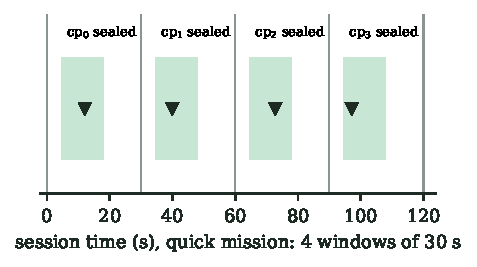
\includegraphics[width=.62\linewidth]{checkin_timing.pdf}
\caption{Check-in timing for a quick mission. Shaded areas are the 15--60\% band where a check can appear, and triangles
are one sample of $\theta_w$. A checkpoint is sealed and sent at each window boundary.}\label{fig:timing}
\end{figure}

\subsection{Physical evidence}\label{sec:physical}
\code{MotionProbe} samples the accelerometer $\mathbf{a}_t=(x_t,y_t,z_t)$ at about 100\,Hz, which is below the 200\,Hz
rate that requires a permission. It keeps a 400-sample ring buffer (about 4\,s). With $m_t=\lVert\mathbf{a}_t\rVert$ it
maintains a slow baseline and a face-down filter:
\begin{equation}
b_t = b_{t-1} + 0.02\,(m_t-b_{t-1}),\qquad \bar z_t=\bar z_{t-1}+0.05\,(z_t-\bar z_{t-1}),\qquad
\textsf{faceDown}_t \iff \bar z_t < -7\ \text{m/s}^2 .
\end{equation}
\emph{Knock.} A knock is registered at sample $t$ if
\begin{equation}\label{eq:knock}
|m_t-b_{t-1}|>\kappa\ \wedge\ t>t_{\text{quiet}}\ \wedge\ t-t_{\text{last knock}}>350\,\text{ms}.
\end{equation}
The threshold is personal. Calibration listens at $0.15$\,m/s$^2$ for three knocks $k_1,k_2,k_3$ and sets
\begin{equation}\label{eq:calib}
\kappa = \max\!\big(0.2,\ \tfrac12\,\mathrm{median}(k_1,k_2,k_3)\big)\ \text{m/s}^2,
\end{equation}
with a default of $\kappa=0.35$\,m/s$^2$. Sensor noise on our test phone measured $\le 0.09$\,m/s$^2$.

\emph{Touch motion $\mu$.} For an on-screen tap at time $t_0$, the baseline is the median of $m$ over
$[t_0-1.5\,\text{s},\,t_0-150\,\text{ms})$, and
\begin{equation}\label{eq:mu}
\mu(t_0)=1000\cdot\max_{t\in[t_0-150\,\text{ms},\ t_0+300\,\text{ms}]}\big|m_t-\mathrm{median}\big(m_{[t_0-1.5\,\text{s},\,t_0-150\,\text{ms})}\big)\big|
\quad[\text{mm/s}^2].
\end{equation}
A knock contributes its own deviation $1000\,|m_t-b_{t-1}|$. Each window reports $\mu_w=\max$ over its answers, or $-1$
if there were none. A finger moves the phone. An \code{adb input tap}, an accessibility gesture or an agent's injected
event does not.

\emph{Stillness $\pi$.} Time is cut into one-second buckets $B$. A bucket \emph{counts} if it has at least 5 samples and
starts more than 2\,s after the last answer, so the knock itself is never held against the user. A counted bucket is
\emph{still} if
\begin{equation}
\mathrm{sd}_{t\in B}(m_t) < 0.08\ \text{m/s}^2\ \wedge\ \mathrm{mean}_{t\in B}(z_t)<-7\ \text{m/s}^2,\qquad
\pi_w=\Big\lfloor 100\,\frac{|\{B\ \text{still}\}|}{|\{B\ \text{counted}\}|}\Big\rfloor .
\end{equation}

\subsection{The server predicate}
Let $t_s$ be the start, $t_u$ the submit time, and $r_0<\dots<r_{K-1}$ the checkpoint receipt times on the server clock,
with $r_{-1}=t_s$. Each checkpoint $i$ carries the foreground flag $f_i$, the answer count $n_i$, the answer time $\lambda_i$
(in ms), $\pi_i$ and $\mu_i$. With tolerance $\delta=3$\,s and achieved assurance $A$, the session passes the policy stage
iff
\begin{align}
C_1&: A\ge A_{\text{req}} &
C_2&: K\ge N &
C_3&: t_u-t_s\ge D-\delta \nonumber\\
C_4&: \forall i:\ r_i-r_{i-1}\ge I-\delta &
C_5&: \forall i:\ f_i=1 &
C_6&: \big|\{i: n_i<n_{\min}\}\big|\le a . \label{eq:pred}
\end{align}
Then three further stages apply, in order:
\begin{align}
C_7&:\ \varrho(\boldsymbol\lambda)<0.9 && \text{(automation risk, \S\ref{sec:risk})}\\
C_8&:\ \forall i:\ n_i>0\Rightarrow \mu_i\ge\tau && \text{(human touch)}\\
C_9&:\ \forall i:\ \pi_i\ge\pi_{\min} && \text{(phone down)}
\end{align}
The verdict is
\[
\text{verdict}=\begin{cases}
\textsc{policy\_not\_satisfied} & \text{if } \neg(C_1\wedge\dots\wedge C_6)\\
\textsc{automation\_detected} & \text{else if } \neg C_7\vee\neg C_8\\
\textsc{policy\_not\_satisfied} & \text{else if } \neg C_9\\
\textsc{verified} & \text{otherwise } (\Pi=\textstyle\bigwedge_{j=1}^{9}C_j)
\end{cases}
\]
Every violated clause in $C_1..C_6$ is listed in the receipt, not just the first. In \emph{development mode} (emulators,
which have no real motion), $C_8$ and $C_9$ are evaluated and reported as \code{FLAGGED} rather than failing the session.
Every receipt carries \code{"mode": "development"}. Development mode is never the default, and a test enforces this.

Two consequences follow directly. From $C_3$ and $C_4$, the minimum server time to a verdict is
$\max(D-\delta,\,N(I-\delta))$, which is 117\,s for the quick mission. From $C_5$, opening any other app in any window
fails the session, regardless of the miss allowance $a$.

\subsection{Automation risk}\label{sec:risk}
Let $R=\{\lambda_i:\lambda_i\ge0\}$ be the answered checks. If $|R|<3$, then $\varrho=0$. Otherwise
\begin{equation}\label{eq:risk}
\phi=\frac{|\{\lambda\in R:\lambda<150\}|}{|R|},\qquad
s(\sigma)=\begin{cases}1 & \sigma<15\\ 0.6 & 15\le\sigma<40\\ 0 & \sigma\ge 40\end{cases},\qquad
\varrho = 1-(1-\phi)\,\big(1-s(\sigma_R)\big),
\end{equation}
where $\sigma_R$ is the population standard deviation of $R$ in ms. The 150\,ms floor comes from simple reaction time to
an unexpected stimulus. The two factors combine like independent detectors (a noisy-OR). The rejection region
$\varrho\ge0.9$ has a closed form:
\begin{equation}
\varrho\ge 0.9\iff \sigma<15\ \ \vee\ \ (15\le\sigma<40\wedge\phi\ge0.75)\ \ \vee\ \ \phi\ge 0.9 .
\end{equation}
Figure~\ref{fig:risk} plots the surface with the devnet prototype's sessions on it. This is a heuristic, not a model. It
catches instant or metronome-steady answers. A script that adds human-like random delays defeats it, and our own
measurements show this (\S\ref{sec:eval}).

\begin{figure}[t]\centering
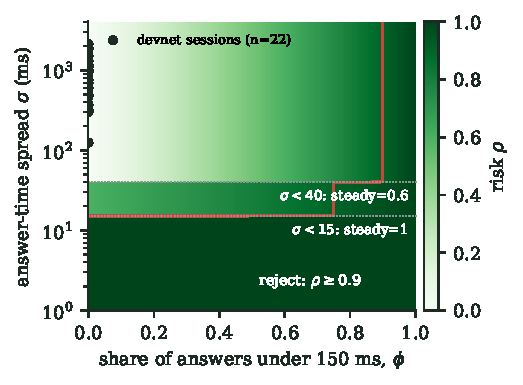
\includegraphics[width=.55\linewidth]{risk_surface.pdf}
\caption{Automation risk $\varrho(\phi,\sigma)$ from Eq.~\eqref{eq:risk}. The red contour is the rejection boundary
$\varrho=0.9$. Dots are the 22 sessions with at least three answers, measured during the earlier devnet prototype. All
have $\phi=0$ and $\sigma\ge125$\,ms, so all score $\varrho=0$, including the sessions driven by \code{adb}.}\label{fig:risk}
\end{figure}

\section{Evidence Chain and Key Binding}\label{sec:evidence}

Let $\|$ denote joining with the byte \code{0x7C} (`$|$'), and let $H$ be SHA-256. With server nonce $\eta$ and session
id $\textit{sid}$:
\begin{align}
h_{-1}&=H(\texttt{"PRESENCE/genesis/v1"}\,\|\,\textit{sid}\,\|\,\eta) \label{eq:gen}\\
p_i&=\texttt{"}i|t^{\text{cl}}_i|e_i|f_i|n_i|\lambda_i|\pi_i|\mu_i\texttt{"}\\
h_i&=H(\texttt{"PRESENCE/cp/v3"}\,\|\,h_{i-1}\,\|\,p_i\,\|\,\eta)\\
\textit{root}&=H(\texttt{"PRESENCE/root/v1"}\,\|\,h_{K-1}\,\|\,0^{32}) \label{eq:root}
\end{align}
The 32 zero bytes are the witness root (P3 not implemented). Here $t^{\text{cl}}_i$ and $e_i$ are the client wall-clock
and elapsed times, which are \emph{informational only}. The domain-separation strings stop a checkpoint hash from being
reused as a genesis or root. Including $\eta$ in every link binds the chain to one session.

\paragraph{Key binding.} At session start the app generates an ephemeral P-256 key in the Android Keystore. Its public
key is embedded in the SIWE (EIP-4361, chain 10143) message that the wallet signs with \code{personal\_sign}. Each
checkpoint is sent as $(p_i, h_i, \mathrm{Sig}_{k}(h_i))$. ATTEST verifies the wallet's EIP-191 signature over the exact
message bytes it issued (the recovered address must be the session's wallet). It then recomputes $h_i$ from $h_{i-1}$ and
$p_i$, verifies the P-256 signature, and stores the chain head. A checkpoint from another session, from a reordered chain
or with an edited field fails one of these three checks. The key is destroyed when the session ends.

\paragraph{Privacy.} Each window discloses one foreground bit, an answer count, one answer time and two motion
summaries. Raw sensor samples stay on the device. There is no location, camera, microphone or contacts access. Only the
32-byte root, the assurance level, and SHA-256 hashes of the identity and the mission reach the chain.

\paragraph{Cross-language determinism.} \code{evidence.py} and \code{EvidenceChain.kt} share golden vectors, so an
independent verifier, such as a future Guardian (\S\ref{sec:future}), can re-derive any root from the receipt.

\section{Settlement and Economics}\label{sec:econ}

\subsection{Three modes}
Let $s$ be the stake, $\beta$ the bonus rate, $w$ the sponsor reward, and \textsf{F}/\textsf{Q} mean finish/quit.

\begin{table}[h]\small\centering
\caption{Payoffs by mode. No cell moves one user's money to another user.}\label{tab:modes}
\begin{tabular}{@{}lccc@{}}\toprule
 & \textbf{Free} & \textbf{No-Loss} & \textbf{Stake (Cool-down)}\\\midrule
At risk & nothing & $s$ locked for the session & $s$ \\
Finish (\textsf{F}) & $+w$ (sponsor) & $s$ back $+\,w$ & $s$ back $+\min(\beta s,\ P-R)$ \\
Quit (\textsf{Q}) & $0$ & $s$ back (refund) & $s$ locked $L(k)$ days, then back \\
Abandoned & $0$ & refunded after expiry & as quit \\\bottomrule
\end{tabular}
\end{table}

\noindent On Monad testnet every amount is in \mon{}. The deployed missions stake 0.05 or 0.2\,\mon{} (No-Loss and
Stake, $\beta=0.2$ for Stake) and pay sponsor rewards of 0.005--0.05\,\mon{} (Free and No-Loss).

\subsection{Pool accounting}
Each mission has a pool with verified sponsor deposits $D_p$ (credited only after ATTEST confirms the deposit
transaction on-chain), forfeits $F_p$ (zero under current rules) and outstanding reservations $R_p$:
\begin{equation}
P_{\text{rem}} = D_p + F_p - R_p .
\end{equation}
A sponsor reward $w$ is reserved at verification only if $P_{\text{rem}}\ge w$. A Stake bonus is
\begin{equation}\label{eq:bonus}
\textit{bonus}=\min\!\big(\operatorname{round}(s\beta),\ \max(P_{\text{rem}},0)\big),
\end{equation}
and the app shows it live before the user commits. By construction, the sum of all payouts never exceeds deposits, and
the operator never needs to mint (Figure~\ref{fig:econ}, left). Rewards are native \mon{} transfers from
\code{PresenceVault} through \code{pay()}, which only the attestor may call. A deposit is credited only if its receipt
carries a \code{Funded} event from the vault. In addition, each device identity can earn at most a fixed sponsor reward
plus bonus per UTC day (\code{DAILY\_REWARD\_CAP\_PER\_DEVICE}); settlement pays $\min(\text{reward},\ \text{cap left
today})$, and returned stakes never count against the cap. Farming one device pays only if $\text{cap}\times\text{days}$
exceeds the device's cost. That is a design argument, not a measurement.

\subsection{Cool-down Lock: loss aversion without forfeiture}
Let $k$ be the number of cool-down locks a wallet has taken in the last 30 days, including this one. The lock length is
\begin{equation}\label{eq:cooldown}
L(k)=\big(7,\ 14,\ 30\big)_{\min(k,3)}\ \text{days}.
\end{equation}
A quitter's stake is never taken. The cost of quitting is the time value of the locked stake. With finishing probability
$p$ and opportunity rate $r$:
\begin{equation}
\mathbb{E}[C_{\text{forfeit}}]=(1-p)\,s,\qquad
\mathbb{E}[C_{\text{cool-down}}]=(1-p)\,s\,\frac{r\,L(k)}{365},\qquad
\frac{\mathbb{E}[C_{\text{cool-down}}]}{\mathbb{E}[C_{\text{forfeit}}]}=\frac{r\,L(k)}{365}.
\end{equation}
At $r=10\%$/yr the ratio is 0.19\% for a 7-day lock and 0.82\% for a 30-day lock (Figure~\ref{fig:cool}). The money cost
is therefore close to zero. The psychological cost, not having access to your money, is what remains. This trades
commitment strength for safety on purpose. Halpern et al.\ found deposits more effective among people who would accept
them, but almost nobody accepted them~\cite{halpern2015}. Derksen et al.\ found most commitment-device takers lost their
money~\cite{derksen2021}. Whether a lock is \emph{enough} commitment is an open empirical question we have not measured.
On Monad the locked stake stays in \code{PresenceVault}; ATTEST returns it with \code{pay()} once the lock has run out.

\begin{figure}[t]\centering
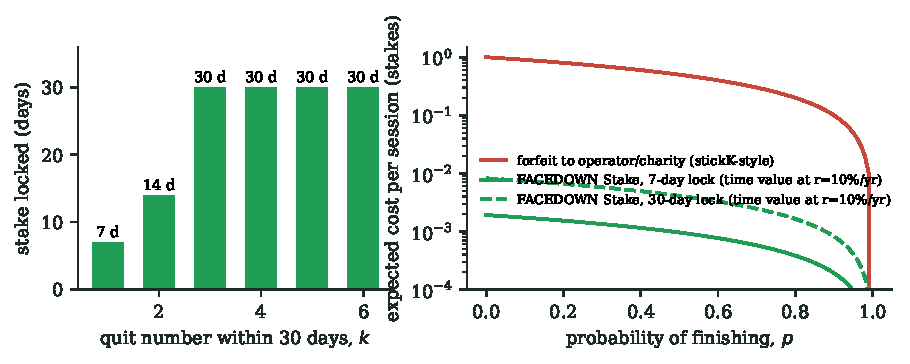
\includegraphics[width=\linewidth]{cooldown.pdf}
\caption{Left: lock length $L(k)$ from Eq.~\eqref{eq:cooldown}. Right: expected money cost per session against the
probability of finishing (log scale). The forfeiture curve is a stickK-style commitment contract. FACEDOWN's Stake cost is
the time value of the locked stake at an illustrative $r=10\%$/yr. No-Loss and Free cost zero (not drawn on a log
axis).}\label{fig:cool}
\end{figure}

\subsection{Streaks, freezes and squads}
Let $\ell$ be the user's last verified UTC day and $\phi_f$ the freezes they hold. A verification on day $d$ updates the
streak $S$ as
\begin{equation}
m=d-\ell-1,\qquad S'=\begin{cases}S+1, & m\le\phi_f\quad(\text{consumes } m \text{ freezes})\\ 1, & \text{otherwise,}\end{cases}
\end{equation}
and the streak is displayed as live while $d_{\text{today}}-\ell\le1+\phi_f$. A freeze has a server-set price
(0.02\,\mon{} on the Monad testnet deployment). The wallet pays it into \code{PresenceVault} with \code{stake(ref)};
the attestor burns half with \code{burn()} (sent to \code{0x\ldots dEaD}) and the other half is protocol revenue. It is
the only sink. A \emph{squad} of $n\le8$ members has one streak, which counts the consecutive days on which \emph{every}
member who had joined by then verified. If each member verifies independently with probability $q$, a squad day succeeds
with probability $q^n$. The chance that a streak survives $d$ days with $f$ freezes is
\begin{equation}\label{eq:survive}
\Pr[\text{alive at }d]=\sum_{j=0}^{f}\binom{d}{j}\,(1-q^n)^j\,(q^n)^{d-j}.
\end{equation}
Figure~\ref{fig:econ} (right) shows the trade-off. A squad of three at $q=0.9$ loses its streak within about two weeks.
At $q=0.97$ it lasts as long as a solo user at $q=0.9$. Squads multiply social pressure and also fragility, which is why
membership is capped at 8 and freezes exist. Eq.~\eqref{eq:survive} is a model (independent days, freezes not
replenished), not a measurement.

\begin{figure}[t]\centering
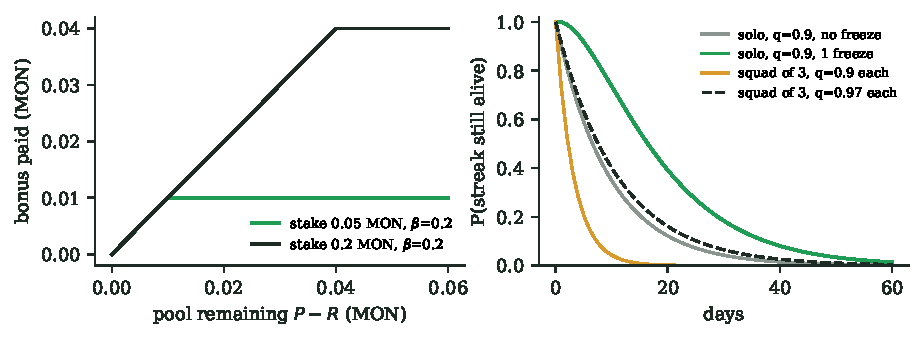
\includegraphics[width=\linewidth]{economics.pdf}
\caption{Left: Stake bonus from Eq.~\eqref{eq:bonus} as the pool drains, for the deployed Stake missions. The
0.05-\mon{} stake saturates at its 0.01 cap; the 0.2-\mon{} stake is limited by the pool up to 0.04. Right: modelled
streak survival from Eq.~\eqref{eq:survive}.}\label{fig:econ}
\end{figure}

\subsection{Stake integrity}
ATTEST issues the stake as an unsigned call $T=(\textit{to}=\text{vault},\ \textit{data}=\code{stake}(\textit{ref}),\
\textit{value}=s)$ with a fresh random 32-byte $\textit{ref}$. The user's wallet (the Privy embedded wallet, as an
EIP-1559 transaction on chain 10143) sends it itself and hands ATTEST the transaction hash. Wallets legitimately choose
their own gas and fees, so ATTEST does not compare transaction bytes. It fetches the receipt and accepts the stake only if
the receipt contains a \code{Staked} event emitted by the vault with
\begin{equation}
\textit{ref}(T')=\textit{ref}(T),\qquad \textit{sender}(T')=\textit{wallet},\qquad \textit{amount}(T')=s .
\end{equation}
A changed amount, recipient, reference or sender produces no matching event and is refused.

\subsection{Why no token and no rake on losers}
Play- and move-to-earn economies pay rewards from emissions and collapse when new deposits slow~\cite{gao2026}.
FACEDOWN has no token. Its rewards are sponsor transfers: parents funding a student, employers funding focus hours, or
protocols funding campaigns. India's Promotion and Regulation of Online Gaming Act (2025) prohibits online money games.
A design where stakers win quitters' stakes risks falling within that definition. Under FACEDOWN's rules (No-Loss
refunds, Stake locks then returns, sponsor-only rewards) no user's money is ever paid to another. That is our reading of
the law, not legal advice, and it needs review before a public launch.

\section{On-Chain Anchoring on Monad}\label{sec:chain}

Five Solidity contracts (355 lines, Foundry) are deployed on Monad testnet and source-verified on Sourcify
(Table~\ref{tab:contracts}).

\begin{table}[h]\small\centering
\caption{Contracts on Monad testnet (chain 10143). Full addresses and transaction hashes are in
\code{contracts/deployments/monad-testnet.json}.}\label{tab:contracts}
\begin{tabular}{@{}ll@{}}\toprule
\code{PresenceRegistry} (v2) & \href{https://testnet.monadvision.com/address/0x5519dacface816519ACa3ee3cD592fd4c61dE52B}{\code{0x5519dacf\ldots E52B}}\\
\code{PresenceVault} & \href{https://testnet.monadvision.com/address/0xfC157D4b8D9573413a3A793056D7625eD972163B}{\code{0xfC157D4b\ldots 163B}}\\
\code{AgentGuard} (limit 0.01\,\mon{}) & \href{https://testnet.monadvision.com/address/0xdC3Ba526FF565D0c76131D54a30aFA3c55041B11}{\code{0xdC3Ba526\ldots 1B11}}\\
\code{SustainedHumanAirdrop} (3 of 30 days) & \href{https://testnet.monadvision.com/address/0x62CbaaAc53ef415fE0262E41e3ce4C2B9af164d1}{\code{0x62CbaaAc\ldots 64d1}}\\
\code{HumanGatedVault} (first demo) & \href{https://testnet.monadvision.com/address/0x2AF710af85914DEe0AA89017223638367645f6b4}{\code{0x2AF710af\ldots f6b4}}\\
Attestor & \code{0x5aB3036C\ldots 4954}\\\bottomrule
\end{tabular}
\end{table}

\subsection{PresenceRegistry}
\code{record(identity, mission, day, seq, root, A)} stores an attestation under
\begin{gather}\label{eq:pda}
\textit{key}=\mathrm{keccak256}\big(\mathrm{abi.encode}(\textit{identity},\ \textit{mission},\ \textit{day},\ \textit{seq})\big),\\
\textit{identity}=H(\text{identity key}),\qquad \textit{mission}=H(\textit{mission\_id}),\nonumber
\end{gather}
and reverts with \code{AlreadyAttested} if that key was written before. A claim index $\textit{seq}<c_{\max}$ that has
already been used therefore cannot be used again, by anyone, ever (G5). The function also requires:
\begin{itemize}
\item the caller is an attestor (\code{isAttestor}, set by the admin);
\item $A\in\{1,2,3,4\}$;
\item $\textit{day}\in\{\lfloor t/86400\rfloor,\ \lfloor t/86400\rfloor-1\}$ on the block timestamp.
\end{itemize}
The contract mirrors the streak with $\Delta=\textit{day}-\ell$: $\Delta=0$ keeps it, $\Delta=1$ adds one, and anything
else resets it to 1. It adds $A$ to reputation and sets the day's bit in a per-identity bitmap. The attestor pays the
gas, so users never need \mon{} to be attested. Contracts read two views:
\begin{itemize}
\item \code{isPresent(identity, minAssurance, maxAgeDays)}: the latest attestation has at least \code{minAssurance} and is
at most \code{maxAgeDays} UTC days old (``is a human here now?'');
\item \code{presentDays(identity, fromDay, toDay)}: the number of distinct UTC days in the range with an attestation
(``does a human keep showing up?'').
\end{itemize}

\paragraph{Settlement order.} ATTEST first sends \code{record()} and waits for its receipt. Only if it confirms does it
send \code{PresenceVault.pay()} with the reward (and returned stake). If \code{record()} reverts, for example with
\code{AlreadyAttested}, settlement fails and nothing is paid. This replaces atomicity with ordering: a failure between
the two transactions can leave a recorded session unpaid, never paid twice. ATTEST sends one transaction at a time per
key, so concurrent settlements cannot reuse a nonce.

\paragraph{PresenceVault.} \code{stake(ref)} (payable) emits \code{Staked(ref, from, amount)}; sponsors call
\code{fund()}. Only the attestor may call \code{pay(to, amount, ref)} and \code{burn(amount)}. The contract therefore
trusts the attestor to follow Table~\ref{tab:modes}; G6 is enforced by ATTEST's rules, not by the vault
(\S\ref{sec:limits}).

\paragraph{Identity.} Claim limits and the daily reward cap are keyed by a device identity, which reaches the chain only
as its SHA-256 hash; the registry never sees a wallet address or device id. In the current testnet deployment, which
runs in development mode, the identity key is the signing wallet (\code{dev:<wallet>}) and every receipt says
\code{DEV\_BYPASS}. Binding the identity to genuine hardware is P4 (\S\ref{sec:future}).

\paragraph{Integration.} Any EVM contract can gate an action with one line:
\begin{center}\code{require(IPresence(registry).isPresent(id, 2, 1), "human presence required");}\end{center} \code{HumanGatedVault} (about 50 lines) does this for an AI
agent's withdrawals: above its limit, a withdrawal reverts with \code{HumanPresenceRequired} unless the owner was
verified present recently. An example quest, ``5 verified facedown sessions'', is one that a bot farm cannot complete
without the motion signal.

\subsection{Sustained presence: SustainedHumanAirdrop}
Proof of personhood checks a human once. \code{presentDays} checks that the same identity keeps showing up, so a farm
must keep every fake identity physically present every day, and its cost grows with identities $\times$ days, the
property formalised as bounded participation~\cite{bpc2026}. \code{SustainedHumanAirdrop.claim(identity, to)}, callable
by the attestor (which knows which wallet owns which identity), pays a fixed amount once per identity, and only if
\begin{equation}
\code{presentDays}(\textit{identity},\ t-W+1,\ t)\ \ge\ N_{\min},
\end{equation}
with $W=30$, $N_{\min}=3$ and 0.005\,\mon{} in the deployed instance.

\subsection{Knock to Approve: a human in the loop for AI agents}\label{sec:agentguard}
\code{AgentGuard} holds an agent's budget. Each account is one phone's P-256 public key $(x,y)$, with account id
$\mathrm{keccak256}(x,y)$; \code{bindDevice} binds it once and it can never be rebound. The agent calls
\code{send(account, to, amount)}:
\begin{itemize}
\item if $\textit{amount}\le\textit{limit}$ (0.01\,\mon{}), the transfer goes through with no human;
\item otherwise the contract creates a pending intent with deadline $t+120$\,s, emits \code{IntentRequested}, and
gives it the id
\[\iota=\mathrm{keccak256}\big(\mathrm{abi.encode}(\text{guard},\ \text{chainid},\ \textit{account},\ \textit{to},\
\textit{amount},\ \textit{nonce}{+}{+})\big).\]
\end{itemize}
The phone lies face-down; when it feels a physical knock it signs $\mathrm{sha256}(\iota)$ with its P-256 key (WebCrypto
in any phone browser, the same curve as Android Keystore and passkeys). ATTEST checks the knock evidence and relays
\code{approve}$(\iota, r, s)$, which only the attestor may call. The contract checks the deadline and verifies
\[
\mathrm{P256.Verify}\big((x,y),\ \mathrm{sha256}(\iota),\ (r,s)\big)
\]
itself, by a static call to Monad's P-256 precompile at \code{0x100} (RIP-7212). A verified intent is marked done and
paid; a forged signature reverts with \code{BadSignature}, an expired one with \code{Expired}, and a replay with
\code{UnknownIntent}. Because $\iota$ commits to the contract, chain, account, recipient, amount and a nonce, a
signature for one intent cannot approve another. ATTEST can relay or withhold an approval, but cannot forge one.
The knock is also recorded in \code{PresenceRegistry}. Browser sensors are weaker evidence than the native app, so these
records use assurance level 1 and FACEDOWN sessions use 2.

\paragraph{The agent's wallet.} The agent is a \emph{Privy server wallet} (\code{0x55215B31\ldots 2271}). A Privy policy
lets it sign transactions only to \code{AgentGuard} on chain 10143; any other destination is refused by Privy with
\code{policy\_violation} and never reaches the chain. The two layers are complementary: Privy bounds \emph{where} the
agent can send, and \code{AgentGuard} bounds \emph{how much} it can send without its human.

\section{Implementation and Evaluation}\label{sec:eval}

\subsection{Implementation}
\begin{table}[h]\small\centering
\caption{Implementation (line counts from the working tree on 15 Oct 2026).}\label{tab:impl}
\begin{tabular}{@{}lllr@{}}\toprule
\textbf{Component} & \textbf{Stack} & \textbf{Responsibility} & \textbf{Lines}\\\midrule
FACEDOWN app & Kotlin, Compose & UI, MotionProbe, EvidenceChain, Privy wallet & $\approx$5,400\\
ATTEST & Python, FastAPI, SQLite & policy, anomaly, identity, pools, Monad, agent relay & $\approx$2,600\\
Contracts & Solidity, Foundry & registry, vault, AgentGuard, airdrop, gated vault & 355\\\midrule
Tests & pytest; Foundry; JUnit & 59 (+2 skipped); 10 (real P-256); 10 & ---\\\bottomrule
\end{tabular}
\end{table}

\subsection{Earlier devnet prototype}
Results 1--3 below come from the earlier prototype, which settled on a devnet; that version is archived in
\code{legacy/solana} and none of these numbers were measured on Monad. Its ATTEST ran in development mode from 9 to 12
October 2026. Clients were a realme RMX3242 (Android~13) with a mobile wallet app, and the Android emulator with a test
wallet. The real phone was connected over USB with \code{adb reverse}; the server was not publicly deployed. Real-phone
sessions were driven by \code{scripts/device\_e2e.py}, which answers check-ins with \code{adb input tap}. This makes them a
direct measurement of an \emph{automated} client on real hardware. Emulator sessions drove knocks and face-down through
the virtual accelerometer. The verification engine (evidence chain, predicate, motion statistics) is the same code that
runs on Monad today.

\begin{table}[h]\small\centering
\caption{Devnet prototype totals (from the prototype's database, regenerated by \code{make\_figures.py}).}\label{tab:deploy}
\begin{tabular}{@{}lr@{\qquad}lr@{}}\toprule
Sessions / wallets & 56 / 20 & Checkpoints sealed / answered & 119 / 95\\
Settled / rejected & 19 / 9 & Rejected: left foreground / missed checks & 7 / 2\\
Active (abandoned) / created only & 3 / 25 & Stakes returned / locked / issued unsigned & 10 / 7 / 13\\
Sponsor deposits verified & 11 & Streak-freeze orders & 3\\
Squads / members & 5 / 7 & Claims recorded & 19\\\bottomrule
\end{tabular}
\end{table}

One stake row is recorded as \textsc{forfeited}. It comes from an earlier build whose rules forfeited a quitter's stake,
before the Cool-down Lock replaced forfeiture. The 25 \textsc{created} sessions were issued a nonce whose sign-in the
wallet never completed.

\begin{figure}[t]\centering
\begin{minipage}{.49\linewidth}\centering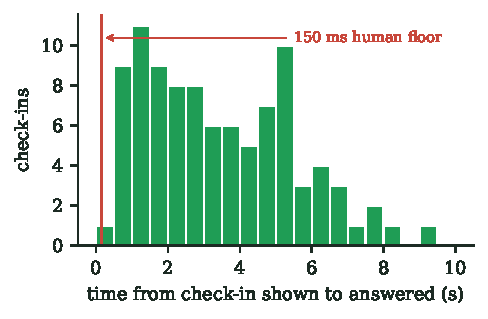
\includegraphics[width=\linewidth]{answer_times.pdf}\end{minipage}\hfill
\begin{minipage}{.49\linewidth}\centering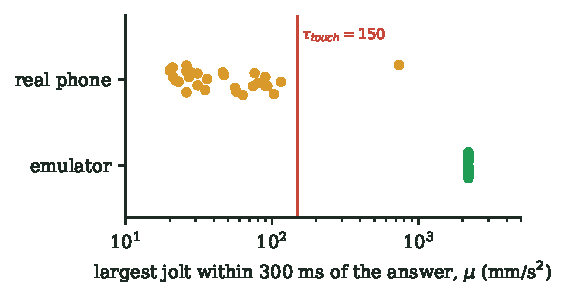
\includegraphics[width=\linewidth]{touch_motion.pdf}\end{minipage}
\caption{Measured during the earlier devnet prototype. Left: the 95 answer times (median 3.07\,s, min 344\,ms). None is
under the 150\,ms floor, so $\phi=0$ everywhere. Right: touch motion $\mu$ by source. Injected taps on the real phone fall
below $\tau$ in 29 of 30 cases. The emulator's synthetic knocks clear it easily.}\label{fig:measured}
\end{figure}

\subsection{Result 1: timing does not detect a script; motion does}
All 22 sessions with $\ge3$ answers scored $\varrho=0$ (Figure~\ref{fig:risk}). This includes the eight real-phone
sessions answered by \code{adb input tap}. Their answer times inherit the latency of the script's UI polling
(\code{uiautomator dump}, then tap) and so look human: none is under 150\,ms, and $\sigma\ge125$\,ms. The motion statistic
separated them. The 30 injected taps read $\mu\in[20,734]$\,mm/s$^2$, median 35.5, and 29 were below $\tau=150$. Every one
of the eight sessions contains a sub-floor answer, so $C_8$ fails for all eight. In development mode, 11 settled receipts
carry \code{human\_touch: FLAGGED} and would have been \textsc{automation\_detected} in production. The single 734 reading
is unexplained. Our working hypothesis is a coincident physical bump to the phone or cable. It shows that one reading
can clear the floor by chance. The rule requires \emph{every} answered window to clear it, so a session-level miss needs
every reading to be lucky.

\subsection{Result 2: injected sensors defeat the motion check}
All five settled sessions whose receipts show both \code{human\_touch} and \code{phone\_down} as \code{PASSED} came from
the emulator. Its virtual accelerometer produced knocks of 2,189--2,190\,mm/s$^2$ (about 15$\times$ the floor) and
stillness of 84--100\%. To the server these are indistinguishable from a person. Any client that can write accelerometer
values (an emulator, a rooted phone, a hooked sensor HAL, or a privileged system-level agent that generates time-aligned
touch and IMU signals~\cite{actreal2026}) passes $C_8$ and $C_9$. This is the strongest attack on the current build.
Only hardware-backed attestation that the app runs unmodified on a genuine device closes it (P4, \S\ref{sec:future}).

\subsection{Result 3: why sessions failed}
Of the 9 rejections, 7 were caused by leaving the foreground ($C_5$) and 2 by missed check-ins beyond $a$ ($C_6$). None
failed on timing ($C_3$, $C_4$): no client in the deployment attempted to compress time.

\subsection{Result 4: Monad testnet deployment}
ATTEST runs on a public host (\url{https://presence-h7uy.onrender.com}) in development mode against the contracts in
Table~\ref{tab:contracts}. Table~\ref{tab:cost} gives the measured cost of anchoring, and Table~\ref{tab:tx} lists
transactions from real phones. These are individual runs, not a population study: we have no Monad-side session totals
comparable to Table~\ref{tab:deploy}.

\begin{table}[h]\small\centering
\caption{Measured on Monad testnet.}\label{tab:cost}
\begin{tabular}{@{}ll@{}}\toprule
Recording one verified session (\code{record()}), 13 Oct 2026 & 161,016 gas, $\approx$0.0164\,\mon{} at 102\,gwei\\
A later \code{record()} transaction, 14 Oct 2026 & 128,512 gas, 0.0131\,\mon{} $\approx$ \$0.0003 at \$0.0244/\mon{}\\
Block time, averaged over 1,000 blocks & 0.304\,s\\\bottomrule
\end{tabular}
\end{table}

\begin{table}[h]\small\centering
\caption{Monad testnet transactions (\href{https://testnet.monadvision.com}{testnet.monadvision.com}).}\label{tab:tx}
\begin{tabularx}{\linewidth}{@{}X l@{}}\toprule
FACEDOWN session, Google sign-in via Privy: embedded wallet signed in-app, 4 knocks, 0.005\,\mon{} sponsor reward &
\tx{0x6e8abfc84566f1026fb800c37d93a1e87362cd85e866ddf0d0786e3b0ad63ee1}{0x6e8abfc8\ldots 3ee1}\\
FACEDOWN No-Loss, Privy: embedded wallet signed the session and the 0.05\,\mon{} stake; 4 knocks; stake back + 0.005\,\mon{} &
\tx{0xe7f5a4159312f0acce7768479d0fe0cad9cece2db374c77c5faf7c71f38b4850}{0xe7f5a415\ldots 4850}\\
FACEDOWN session from the phone app with MetaMask sign-in, 4 knock check-ins &
\tx{0xe07ccaa13b6a2d2c381a9a455a7dd99e48509c68e9cb5d2337c5453412c759c4}{0xe07ccaa1\ldots 59c4}\\
Knock to Approve on a real phone (Chrome): agent's 0.03\,\mon{} held / two knocks, P-256 verified on-chain, sent &
\tx{0x43e97991cc252267a32d5cb8cad21b497b74bbb14f714c4556bd619b496c30fc}{0x43e97991\ldots 30fc} /
\tx{0xd150e895b85e060228b06d7388b84192116b502eea9fa78fb90e2c3bd943b533}{0xd150e895\ldots b533}\\
Knock to Approve, scripted: phone key bound / agent (signed by Privy) sends 0.005\,\mon{}, no approval &
\tx{0x41bd309df3eb8168f0ec604d5bb3551fe68e4732572fd06ad32c73f713d80439}{0x41bd309d\ldots 0439} /
\tx{0xaa726c9cdf881b438c162ef28fe3055a7865a3bf6034b26d426209ac8aa3ff84}{0xaa726c9c\ldots ff84}\\
\quad agent sends 0.03\,\mon{}, held / P-256 verified, sent / presence recorded &
\tx{0xa33e7f59a14f99c57a6f6f7a7c49a9bf4e4a7b89c41466e4bf09f9b92b683e59}{0xa33e7f59\ldots 3e59} /
\tx{0x0881af9d492b67d1edf291bb93bffb2130ff1f2f36eb7f0c5dcde2e6c4a8f9b2}{0x0881af9d\ldots f9b2} /
\tx{0x3dcaa0a3185f0a0941aa4d638a58afdf8f3a938fd2753b501adef71f253d0365}{0x3dcaa0a3\ldots 0365}\\
\quad agent asks Privy to sign a transfer to another address & refused, \code{policy\_violation}\\
\code{HumanGatedVault}: agent withdrawal blocked / presence recorded / withdrawal allowed &
\tx{0xe257dd0baf4eacc1ea37ef191e27f8a75d3f4d548d23e83275977d06961970dc}{0xe257dd0b\ldots 70dc} /
\tx{0xa0466d10fb58ae4c9fcfbc52360f234bf0b99c49fde663b2e31991fa85348e52}{0xa0466d10\ldots 8e52} /
\tx{0x1d1befe4e297cfef6b0924e3be01f7ac998f0f33dd6117929f53a4868d873bf4}{0x1d1befe4\ldots 3bf4}\\\bottomrule
\end{tabularx}
\end{table}

\subsection{Verifier cost}
Table~\ref{tab:lat} reports the time to recompute the chain and root (Eqs.~\eqref{eq:gen}--\eqref{eq:root}) and evaluate the full predicate
(clauses $C_1$--$C_9$), over 2,000 runs on an Intel i5-13420H with CPython 3.14. Cost is linear in $K$. Repeated runs vary by about 10\%; the table is the run saved in \code{measured.json}. Verification is
negligible next to on-chain confirmation (0.304\,s blocks on Monad, and ATTEST polls receipts every 0.5\,s), so the
engine's throughput is bounded by RPC and database I/O, not cryptography.

\begin{table}[h]\small\centering
\caption{Chain recompute and policy evaluation latency (measured).}\label{tab:lat}
\begin{tabular}{@{}rrr@{}}\toprule
Checkpoints $K$ & p50 (\textmu s) & p99 (\textmu s)\\\midrule
4 & 16.4 & 37.9\\ 16 & 31.4 & 56.3\\ 64 & 85.8 & 191.8\\ 256 & 259.5 & 437.3\\ \bottomrule
\end{tabular}
\end{table}

\subsection{What a cheater would try}
Table~\ref{tab:attacks} lists every attack we considered and how far each defence has been exercised.
\begin{table}[H]\small
\caption{Attacks and their status. ``Reproduced'' means observed in a deployment; ``tested'' means covered by the
backend or Foundry test suite.}\label{tab:attacks}
\begin{tabularx}{\linewidth}{@{}l X l@{}}\toprule
\textbf{Attempt} & \textbf{Why it fails} & \textbf{Status}\\\midrule
Fast-forward the timer & $C_3$, $C_4$ on the server clock & tested\\
Use the phone mid-session & $C_5$ foreground bit; $C_9$ stillness & reproduced (7 rejections, devnet)\\
Script / AI agent answers & $C_8$: injected input has no jolt & reproduced (30 taps, 8 sessions, devnet)\\
Replay or forge evidence & nonce in every link; P-256 sig per checkpoint & tested\\
Many wallets, one device & claims keyed by device identity hash & tested; dev mode keys by wallet\\
Swap the stake tx in the wallet & receipt must hold \code{Staked}(ref, sender, exact amount) from the vault & by construction\\
Claim the payout twice & create-once record; payout only after it confirms & tested (\code{AlreadyAttested})\\
Agent sends above its limit & intent waits for the phone's P-256 signature & reproduced on Monad; tested\\
Relay forges or reuses an approval & on-chain P-256 check over $\iota$; 120\,s expiry; done flag & reproduced (forged sig); tested\\
Agent signs a transfer elsewhere & Privy policy: only \code{AgentGuard} on chain 10143 & reproduced (\code{policy\_violation})\\
\textbf{Inject sensor values} & \textbf{not defended (needs P4)} & \textbf{reproduced (emulator)}\\
Second phone & not defended (non-goal) & ---\\\bottomrule
\end{tabularx}
\end{table}

\section{Findings from Testing on Real Phones}\label{sec:findings}
\begin{enumerate}
\item \textbf{An external wallet hop breaks the session clock.} With MetaMask, the app opens ATTEST's signing page in
MetaMask's own browser (\code{metamask://} deep link), and that browser cannot open other apps, so the user returns
through a notification. Check-ins queued while the user was in the wallet, and a session was rejected. The session clock
now starts when the user is back in FACEDOWN; the app may only move the start later, and only before the first
checkpoint. Google sign-in through Privy removes the hop: the embedded wallet signs the SIWE message and the stake
transaction inside the app.
\item \textbf{Monad bills the gas limit.} ATTEST sets the limit to $1.2\times$ the estimate ($1.1\times$ for agent
transactions) rather than a generous fixed value.
\item \textbf{Public RPCs rate-limit.} The testnet RPC answers HTTP 429 under load; ATTEST retries with backoff (0.5, 1,
2, 4\,s) and sends one transaction at a time per key so nonces never collide.
\item \textbf{One knock must mean one approval.} On the web Knock-to-Approve page, motion listeners left over from
earlier presses of \emph{Start} fired a second approval for one knock. The page now tears them down; the contract would
have rejected the duplicate anyway (\code{UnknownIntent}).
\item \textbf{Response-time statistics cannot see scripted UI drivers.} See Result 1. The heuristic stays as a cheap
filter for naive bots. The motion floor carries the real weight.
\item \textbf{Emulators stop delivering sensor events when the screen is off.} Presence Minutes (the passive face-down
ring) and Urge Catcher were therefore verified only on the emulator with the screen on. Screen-off sampling on real
phones still needs checking.
\item \textbf{OEMs differ.} realme blocks enabling an accessibility service over \code{adb}, so Urge Catcher must be
switched on by hand in Settings.
\end{enumerate}

\section{Trust Assumptions and Limitations}\label{sec:limits}
Ordered by severity.
\begin{enumerate}
\item \textbf{Sensor injection.} A modified OS, an emulator, a hooked sensor HAL or a privileged system-level
agent~\cite{actreal2026} can produce $\pi$ and $\mu$ that pass. Reproduced. The motion check stops UI-level automation
(scripts, accessibility, AI agents), not a modified device.
\item \textbf{Single operator.} One ATTEST server holds the attestor key. \code{PresenceRegistry} accepts several
attestor addresses (\code{setAttestor}), but one is configured, and \code{PresenceVault}, \code{AgentGuard} and
\code{SustainedHumanAirdrop} each trust a single attestor. A compromised or dishonest operator can attest anything and
can pay any address from the vault: principal safety (G6) rests on ATTEST's rules, not on the contract. For Knock to
Approve, the operator cannot \emph{approve} a transfer without the phone's key, but can withhold approvals. Mitigation
is a Guardian quorum (\S\ref{sec:future}), which is designed but deliberately has no code stub.
\item \textbf{AgentGuard's limit is per transfer, not a budget.} An agent may call \code{send} repeatedly with amounts
at or below the limit, so a compromised agent can drain the guard's balance in 0.01\,\mon{} steps (Privy's policy still
confines it to \code{AgentGuard}). The guard also pays from one shared balance rather than per-account balances. It is a
testnet demonstration; a rate limit and per-account accounting are future work.
\item \textbf{Client-side randomness.} $\theta_w$ in Eq.~\eqref{eq:prompt} is drawn on the phone. A modified client knows
when checks will appear. This matters only together with item 1, because answers still need a physical jolt.
\item \textbf{Real knocks not yet measured across phones.} Knock detection and face-down were measured on the emulator's
virtual sensor in the devnet prototype, and real-phone knocks on Monad are individual runs (Table~\ref{tab:tx}). A
calibrated table of real knocks across phones and surfaces is the next measurement. Until it exists, the
150\,mm/s$^2$ floor is a design value. All we know is that injected taps on a real phone read well below it
(20--115\,mm/s$^2$, one outlier at 734) and synthetic knocks well above it.
\item \textbf{No hardware-bound device identity yet.} The testnet deployment runs in development mode: identities are
keyed by wallet, and every receipt is \code{DEV\_BYPASS}. Until P4, one person with many wallets is not limited per
physical device. Web Knock-to-Approve evidence is weaker still and is recorded at assurance 1.
\item \textbf{This phone, not this person.} We prove a device lay face-down with someone answering it, not who that was or
that they had no other phone. In No-Loss, cheating only cheats yourself. In sponsored pools the per-identity claim limit
and daily reward cap bound what one identity can take.
\item \textbf{Settlement is two transactions.} A failure between \code{record()} and \code{pay()} leaves a recorded session
unpaid until it is retried by hand (\S\ref{sec:chain}).
\item \textbf{Behavioural effect unmeasured.} We cite trials of related interventions, but we have not run one. The
benefit of FACEDOWN itself is unproven.
\item \textbf{Legal.} The design is meant to stay outside India's online money game definition. That is untested and
needs counsel.
\item \textbf{Testnet only.} Everything ran on Monad testnet with testnet \mon{} (and, in the earlier prototype, a
valueless test token), with a development-only faucet. There are no customers yet.
\end{enumerate}

\section{Related Work}
\textbf{Commitment devices.} Deposit contracts work for those who take them up, but uptake is low~\cite{halpern2015}.
Appointments achieve commitment without loss~\cite{derksen2021}, and group pools amplify incentives~\cite{kullgren2013}.
Commercial commitment-contract services verify with referees or self-report and send forfeits to a charity or the
operator. PRESENCE replaces the referee with server-checked sensor evidence and removes the forfeit.
\textbf{Digital well-being.} Focus timers that grow a virtual tree on the device, and app blockers, rely on local state.
The one-sec nudge shows that a pause reduces openings~\cite{gruning2023}. Blocking mobile internet improves
attention~\cite{castelo2025}, and self-chosen goals outperform assigned ones~\cite{sachdeva2026}.
\textbf{Humanness from sensors.} zkSENSE classifies motion during interaction and wraps the result in a zero-knowledge
proof~\cite{zksense}. Liu and Huang show agent-driven MFA completing end to end, and a motion signal that separates it
from humans~\cite{liu2026}. ActReal shows that a privileged system-level agent can generate time-aligned touch and IMU
signals that evade such detectors~\cite{actreal2026}, which is our limitation 1. PRESENCE uses a deliberately simpler,
inspectable statistic, and places it inside a signed, hash-chained process record with an economic outcome. That record
is what makes the signal settle money rather than only score risk.
\textbf{Proof of personhood and sustained participation.} Proof-of-personhood systems establish once that an identity is
a unique human; PRESENCE does not, and is complementary: it shows that a body was at this device just now, and through
\code{presentDays}, that it keeps coming back. The Bounded Participation Channel formalises why re-earned, per-window
participation imposes a linear cost on sustaining many identities~\cite{bpc2026}.
\textbf{Token incentive economies.} Emission-funded play-to-earn games left most trading players at a loss~\cite{gao2026}.
That is the reason for sponsor-only rewards.

\section{Future Work}\label{sec:future}
\begin{enumerate}
\item \textbf{P4 hardware attestation.} Require Android Key Attestation for the ephemeral key, and a platform integrity
verdict, as a policy clause, and derive the device identity from it. This closes limitations 1 and 6.
\item \textbf{Guardian quorum.} Replace the single attestor with a set $G$ of Guardian keys and a threshold $m$. Each
Guardian runs its own ATTEST over the same evidence (the chain is deterministic) and signs $M_g$ below.
\code{record} then accepts iff
\[M_g=(\textit{identity},\textit{mission},\textit{day},\textit{seq},\textit{root}),\qquad
\big|\{g\in G:\mathrm{ecrecover}(M_g,\sigma_g)=g\}\big|\ge m .\]
Guardians stake \mon{} behind their signatures and can be slashed.
\item \textbf{AgentGuard budgets.} Per-account balances and a rolling spend limit, so the no-human allowance is a budget,
not a per-transfer cap (limitation 3).
\item \textbf{P3 witnesses.} Fresh-challenge BLE co-presence witnesses fill the reserved 32-byte witness root.
\item \textbf{Server-issued challenges.} Move $\theta_w$ to the server: it reveals each window's check-in time only at
that moment. This closes limitation 4.
\item \textbf{A learned presence model.} Replace the hand-set thresholds with an on-device classifier trained on opt-in
real traces. We have not built it yet because we have no data to train it on.
\item \textbf{Yield-funded No-Loss.} On mainnet, locked stakes earn lending yield (for example a lending vault on Monad)
that funds the finisher reward in place of sponsors.
\item \textbf{A randomised trial.} Measure whether verified sessions reduce daily screen time compared with an unverified
timer.
\end{enumerate}

\section{Conclusion}
A phone cannot prove that you were focused. It can prove something narrower and still useful: that it lay face-down and
still, that it stayed in one app, and that something physical answered it at moments it chose. The server checks all of
this on its own clock and records it once on Monad, where any contract can ask whether a human is here now and whether
one keeps showing up. Our measurements show where that proof holds and where it does not. It stopped every scripted UI
session we ran on real hardware. It does not stop a device that lies about its own sensors. The same knock now gates AI
agents: above its limit, an agent's transfer waits for a signature that only its human's phone can give, checked by the
contract itself. The economics avoid the two failure modes of earlier designs: forfeits that enrich the operator, and
emissions that collapse. FACEDOWN is the first consumer of PRESENCE. The broader product is proof that a human performed a
process, which every airdrop, quest, reward program and agent wallet currently lacks.

\begin{thebibliography}{99}\small
\bibitem{castelo2025} N.~Castelo, K.~Kushlev, A.~F.~Ward, M.~Esterman, et al. Blocking mobile internet on smartphones
improves sustained attention, mental health, and subjective well-being. \emph{PNAS Nexus} 4(2):pgaf017, 2025.
doi:10.1093/pnasnexus/pgaf017.
\bibitem{halpern2015} S.~D.~Halpern, B.~French, D.~S.~Small, K.~Saulsgiver, et al. Randomized trial of four
financial-incentive programs for smoking cessation. \emph{N Engl J Med} 372:2108--2117, 2015. doi:10.1056/NEJMoa1414293.
\bibitem{sachdeva2026} A.~Sachdeva, J.~Somasundaram, K.~K.~Sharma. Self-selected goals outperform assigned goals in
reducing mobile phone usage: evidence from a randomized controlled trial. \emph{Soc Sci Med} 406:119683, 2026.
doi:10.1016/j.socscimed.2026.119683.
\bibitem{gruning2023} D.~J.~Grüning, F.~Riedel, P.~Lorenz-Spreen. Directing smartphone use through the self-nudge app
one sec. \emph{PNAS} 120:e2213114120, 2023. doi:10.1073/pnas.2213114120.
\bibitem{kullgren2013} J.~T.~Kullgren, A.~B.~Troxel, G.~Loewenstein, D.~A.~Asch, et al. Individual- versus group-based
financial incentives for weight loss: a randomized, controlled trial. \emph{Ann Intern Med} 158:505--514, 2013.
doi:10.7326/0003-4819-158-7-201304020-00002.
\bibitem{derksen2021} L.~Derksen, J.~Kerwin, N.~Ordaz Reynoso, O.~Sterck. Appointments: a more effective commitment
device for health behaviors. arXiv:2110.06876, 2021.
\bibitem{liu2026} Y.~Liu, H.~Huang. WiP: Characterizing and defending against mobile-agent-driven MFA automation.
arXiv:2609.02154, 2026.
\bibitem{zksense} I.~Querejeta-Azurmendi, P.~Papadopoulos, M.~Varvello, A.~Nappa, J.~Zhang, B.~Livshits. ZKSENSE: a
friction-less privacy-preserving human attestation mechanism for mobile devices. arXiv:1911.07649, 2019.
\bibitem{gao2026} Y.~Gao, F.~Li, R.~Shi, R.~Cheng, J.~Zhang, B.~Han, S.~Chen. NFT games: an empirical look into the
play-to-earn model. arXiv:2602.13882, 2026.
\bibitem{bpc2026} H.~Maleki, N.~Sainz, J.~Legarda, I.~Santos-Grueiro. Sustained participation as a security resource:
the bounded participation channel. arXiv:2609.35300, 2026.
\bibitem{actreal2026} M.~Wang, H.~Guo, H.~Li, Y.~Fu, J.~Xu, C.~Xu. ActReal: system-level mobile agents challenge mobile
automation detection. arXiv:2608.30038, 2026.
\end{thebibliography}

\vspace{6pt}
\noindent\rule{\linewidth}{.4pt}\\
\small\emph{Every number in this paper was measured from the code, the test suite, the earlier devnet prototype's
database, or Monad testnet, or is quoted from a cited abstract. Figures~\ref{fig:cool} and~\ref{fig:econ} are labelled
models. Nothing here ran on mainnet; all value is testnet \mon{} (the prototype used a valueless test token). To
reproduce the figures and Tables~\ref{tab:deploy} and~\ref{tab:lat}, the prototype database is required:
\code{uv run --with matplotlib --with numpy python docs/whitepaper/make\_figures.py}.}
\end{document}
